\documentclass[aspectratio=169,12pt]{beamer}
\usepackage[utf8]{inputenc}
\usepackage{graphicx}
\usepackage{tikz}
\usepackage{array}
\usepackage{booktabs}
\usepackage{colortbl}
\usepackage{xcolor}

\usetikzlibrary{shapes,arrows,positioning,shadows,calc}

% Theme
\usetheme{Madrid}
\usecolortheme{default}

% Colors
\definecolor{darkblue}{RGB}{0,51,102}
\definecolor{lightblue}{RGB}{102,153,204}
\definecolor{orange}{RGB}{255,102,0}
\definecolor{lightgray}{RGB}{240,240,240}

\setbeamercolor{structure}{fg=darkblue}
\setbeamercolor{frametitle}{bg=darkblue,fg=white}
\setbeamercolor{title}{bg=darkblue,fg=white}

% Title page
\title[Dal Modello E-R allo Schema Logico]{Dal Modello Entità-Relazione allo Schema Logico}
\subtitle{Progettazione di Database}
\author{Prof. Fedeli Massimo}
\institute{ITS 4.0 - Tutti i diritti riservati}
\date{A.S. 2025/26}

\begin{document}
	
	% Slide 1 - Title
	\begin{frame}
		\titlepage
	\end{frame}
	
	% Slide 2 - Table of Contents
	\begin{frame}{Contenuti}
		\tableofcontents
	\end{frame}
	
	\section{Introduzione alla Progettazione Logica}
	
	% Slide 3
	\begin{frame}{Progettazione Logica: Obiettivo}
		\begin{block}{Obiettivo}
			Costruire uno \textbf{schema logico} in grado di descrivere, in maniera corretta ed efficiente, tutte le informazioni contenute nello schema Entità-Relazione prodotto nella fase di progettazione concettuale.
		\end{block}
		
		\vspace{0.5cm}
		
		\begin{alertblock}{Importante}
			Non è una semplice traduzione da un modello a un altro!
		\end{alertblock}
	\end{frame}
	
	% Slide 4
	\begin{frame}{Progettazione Logica: Ristrutturazione}
		Prima di passare allo schema logico, lo schema E-R va \textbf{ristrutturato} per:
		
		\begin{enumerate}
			\item \textcolor{orange}{\textbf{Semplificare}} la traduzione
			\item \textcolor{orange}{\textbf{Ottimizzare}} il progetto
		\end{enumerate}
		
		\vspace{0.5cm}
		
		\begin{block}{Ricorda}
			La progettazione concettuale ha come obiettivo la rappresentazione accurata e naturale dei dati dal punto di vista del \textit{significato}.
		\end{block}
	\end{frame}
	
	% Slide 5
	\begin{frame}{Progettazione Logica: Base per l'Applicazione}
		\begin{columns}
			\begin{column}{0.6\textwidth}
				La progettazione logica costituisce la \textcolor{orange}{\textbf{base per l'effettiva realizzazione dell'applicazione}} e deve tener conto, per quanto possibile, delle sue \textcolor{darkblue}{\textbf{prestazioni}}.
				
				\vspace{0.5cm}
				
				Questa necessità può portare a una \textbf{ristrutturazione} dello schema concettuale che renda più efficiente l'esecuzione delle operazioni previste.
			\end{column}
			\begin{column}{0.4\textwidth}
				\begin{tikzpicture}[node distance=1.2cm, every node/.style={rectangle, draw, rounded corners, font=\small, text centered, minimum height=0.7cm}]
					\node[fill=lightblue!30, width=2.8cm] (er) {Schema E-R};
					\node[fill=orange!30, width=2.8cm, below=of er] (app) {Carico applicativo};
					\node[fill=lightgray, width=2.8cm, below right=0.2cm and 0.5cm of er] (log) {Modello logico};
					
					\draw[->, thick, darkblue] (er.east) -- (log.west);
					\draw[->, thick, darkblue] (app.east) -- (log.west);
				\end{tikzpicture}
			\end{column}
		\end{columns}
	\end{frame}
	
	% Slide 6
	\begin{frame}{Le Due Fasi}
		È necessario prevedere:
		\begin{enumerate}
			\item Un'attività di \textcolor{orange}{\textbf{riorganizzazione}}
			\item Un'attività di \textcolor{darkblue}{\textbf{traduzione}}
		\end{enumerate}
		
		\vspace{0.5cm}
		
		La progettazione logica si articola quindi in \textbf{due fasi}:
		\begin{itemize}
			\item \textbf{Ristrutturazione} dello schema Entità-Relazione
			\item \textbf{Traduzione} verso il modello logico
		\end{itemize}
	\end{frame}
	
	% Slide 7
	\begin{frame}{Processo di Progettazione}
		\begin{center}
			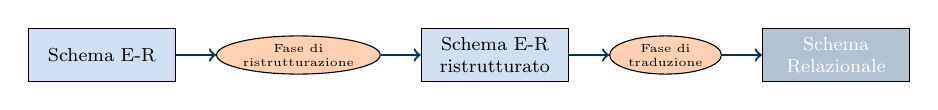
\begin{tikzpicture}[node distance=1cm, scale=0.85, transform shape, 
				box/.style={rectangle, draw, fill=lightblue!30, minimum width=2.2cm, minimum height=0.8cm, font=\footnotesize, align=center},
				phase/.style={ellipse, draw, fill=orange!30, font=\tiny, align=center, inner sep=1pt}]
				\node[box] (er1) {Schema E-R};
				\node[phase, right=0.6cm of er1] (rist) {Fase di\\ristrutturazione};
				\node[box, right=0.6cm of rist] (er2) {Schema E-R\\ristrutturato};
				\node[phase, right=0.6cm of er2] (trad) {Fase di\\traduzione};
				\node[box, fill=darkblue!30, text=white, right=0.6cm of trad] (rel) {Schema\\Relazionale};
				
				\draw[->, thick, darkblue] (er1) -- (rist);
				\draw[->, thick, darkblue] (rist) -- (er2);
				\draw[->, thick, darkblue] (er2) -- (trad);
				\draw[->, thick, darkblue] (trad) -- (rel);
			\end{tikzpicture}
		\end{center}
	\end{frame}
	
	% Slide 8
	\begin{frame}{Output della Progettazione Logica}
		\begin{columns}
			\begin{column}{0.5\textwidth}
				Costituiscono i prodotti finali:
				\begin{itemize}
					\item \textbf{Lo schema logico finale}
					\item \textbf{I vincoli di integrità} definiti su di esso
					\item \textbf{La relativa documentazione}
				\end{itemize}
			\end{column}
			\begin{column}{0.5\textwidth}
				\begin{block}{Esempio}
					\small
					\texttt{Musei(CodiceMuseo, Denominazione, Città, Indirizzo, NumeroOpere)}
				\end{block}
			\end{column}
		\end{columns}
	\end{frame}
	
	% Slide 9
	\begin{frame}{Il Modello Logico}
		Il \textbf{modello logico} del database (o schema logico) è lo strumento che viene utilizzato come \textit{input} per la \textcolor{orange}{\textbf{progettazione fisica}} dei database.
		
		\vspace{0.5cm}
		
		Deve quindi avere il \textcolor{darkblue}{\textbf{massimo livello di dettaglio e precisione possibile}}.
		
		\vspace{0.5cm}
		
		\begin{alertblock}{Funzioni del Modello Logico}
			Dota i dati di una struttura utile per \textbf{realizzare}, \textbf{semplificare} e \textbf{ottimizzare} le operazioni di archiviazione, interrogazione e manipolazione dei dati.
		\end{alertblock}
	\end{frame}
	
	% Slide 10
	\begin{frame}{Modello Logico: Contenuti}
		Deve contenere tutte le informazioni necessarie per \textbf{definire fisicamente le tabelle}, riportando la \textcolor{orange}{\textbf{descrizione puntuale e completa}} del significato di ogni dato che viene memorizzato.
		
		\vspace{0.5cm}
		
		\begin{block}{Esempio Schema Relazionale}
			\texttt{alunni (matricola(pk), cognome, nome, ..., scuola(fk))}
		\end{block}
		
		\vspace{0.3cm}
		
		Questo può essere considerato come \textit{schema logico}, ma è sempre preferibile realizzare un \textcolor{darkblue}{\textbf{modello logico preciso}} (o completo) per rendere più semplice la progettazione fisica.
	\end{frame}
	
	\section{Modello Logico Preciso}
	
	% Slide 11
	\begin{frame}{Componenti del Modello Logico Preciso}
		Un modello logico preciso comprende:
		\begin{enumerate}
			\item Per ogni \textbf{entità}, l'elenco completo degli attributi
			\item Per ogni \textbf{entità}, l'indicazione esplicita della chiave primaria e di eventuali chiavi alternative
			\item Per ogni \textbf{entità}, l'indicazione esplicita di eventuali chiavi esterne
			\item Per ogni \textbf{attributo}, l'indicazione esplicita di opzionalità o obbligatorietà
		\end{enumerate}
	\end{frame}
	
	% Slide 12
	\begin{frame}{Componenti del Modello Logico Preciso (2)}
		\begin{enumerate}
			\setcounter{enumi}{4}
			\item Per ogni \textbf{attributo}, l'indicazione esplicita del tipo di dati (\textit{data type}), che ne specifichi il formato e la lunghezza, con la segnalazione dei valori ammessi
			\item Per ogni \textbf{relazione}, l'indicazione della molteplicità minima e massima in entrambe le direzioni
			\item Per ogni \textbf{relazione}, l'indicazione delle regole di integrità referenziale applicabili
		\end{enumerate}
	\end{frame}
	
	% Slide 13
	\begin{frame}{Esempio: Modello Logico Preciso}
		\begin{center}
			\small
			\begin{tabular}{|l|l|c|l|l|}
				\hline
				\rowcolor{lightblue!50}
				\textbf{Attributo} & \textbf{Tipo} & \textbf{Dim.} & \textbf{Valori} & \textbf{Note} \\
				\hline
				Matricola & Numerico & 8 & Autoincrement & PK \\
				\hline
				Cognome & Stringa & 40 & Not null & \\
				\hline
				Nome & Stringa & 30 & Not null & \\
				\hline
				Scuola & Numerico & 12 & Cod. MIUR & FK \\
				\hline
			\end{tabular}
		\end{center}
		
		\vspace{0.3cm}
		Durante la progettazione logica si definiscono inoltre gli \textcolor{orange}{\textbf{schemi esterni (viste)}} per le specifiche applicazioni.
	\end{frame}
	
	\section{Ristrutturazione dello Schema E-R}
	
	% Slide 14
	\begin{frame}{Ristrutturazione: Panoramica}
		Una volta che lo schema E-R è stato completamente definito, si procede al suo \textbf{affinamento} (ristrutturazione) attraverso:
		
		\vspace{0.5cm}
		
		\begin{block}{Regola Base}
			\textbf{Eliminazione dei costrutti non rappresentabili} applicando delle regole base di modellizzazione
		\end{block}
	\end{frame}
	
	% Slide 15
	\begin{frame}{Eliminazione Costrutti: Entità Scollegate}
		\begin{columns}
			\begin{column}{0.6\textwidth}
				Le \textbf{entità non possono} essere modellate se sono \textcolor{red}{\textbf{scollegate}} da altre entità.
				
				\vspace{0.5cm}
				
				\begin{block}{Eccezione}
					Un database formato da una \textit{singola tabella} (esempio: carrello elettronico nei siti di commercio elettronico)
				\end{block}
			\end{column}
			\begin{column}{0.4\textwidth}
				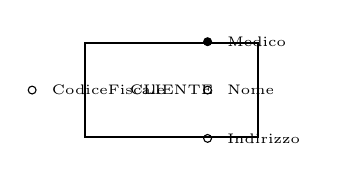
\begin{tikzpicture}[scale=0.8, every node/.style={font=\tiny}]
					\node[rectangle, draw, minimum width=2.2cm, minimum height=1.2cm, thick] (cliente) {CLIENTE};
					\node[circle, draw, fill=black, inner sep=1pt, left=0.6cm of cliente.north east] (p1) {};
					\node[circle, draw, inner sep=1pt, left=0.6cm of cliente.east] (p2) {};
					\node[circle, draw, inner sep=1pt, left=0.6cm of cliente.west] (p3) {};
					\node[circle, draw, inner sep=1pt, left=0.6cm of cliente.south east] (p4) {};
					
					\node[right=2pt of p1] {Medico};
					\node[right=2pt of p2] {Nome};
					\node[right=2pt of p3] {CodiceFiscale};
					\node[right=2pt of p4] {Indirizzo};
				\end{tikzpicture}
			\end{column}
		\end{columns}
	\end{frame}
	
	% Slide 16
	\begin{frame}{Eliminazione Attributi Composti}
		Nel caso fosse presente un \textbf{attributo composto} si può procedere in due modi alternativi:
		
		\begin{enumerate}
			\item \textcolor{darkblue}{\textbf{Considerare}} tutti i sottoattributi come attributi
			\item \textcolor{orange}{\textbf{Eliminare}} i sottoattributi e considerare l'attributo composto come un attributo semplice
		\end{enumerate}
		
		\vspace{0.5cm}
		\begin{center}
			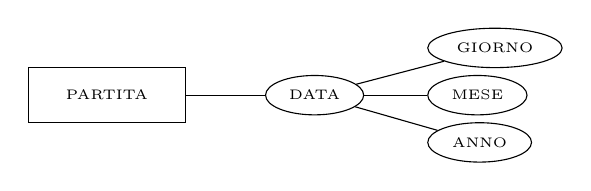
\begin{tikzpicture}[scale=0.9, every node/.style={font=\tiny}]
				\node[rectangle, draw, minimum width=2cm, minimum height=0.7cm] (partita) {PARTITA};
				\node[ellipse, draw, right=1cm of partita] (data) {DATA};
				\node[ellipse, draw, right=0.8cm of data, yshift=0.6cm] (g) {GIORNO};
				\node[ellipse, draw, right=0.8cm of data] (m) {MESE};
				\node[ellipse, draw, right=0.8cm of data, yshift=-0.6cm] (a) {ANNO};
				
				\draw (partita) -- (data);
				\draw (data) -- (g);
				\draw (data) -- (m);
				\draw (data) -- (a);
			\end{tikzpicture}
		\end{center}
	\end{frame}
	
	% Slide 17
	\begin{frame}{Attributi Composti: Soluzione A}
		\textbf{Soluzione A: scomposizione}
		
		\vspace{0.3cm}
		
		Nell'entità \texttt{studente} è presente come attributo composto il \texttt{nr\_telefono}.
		
		\begin{center}
			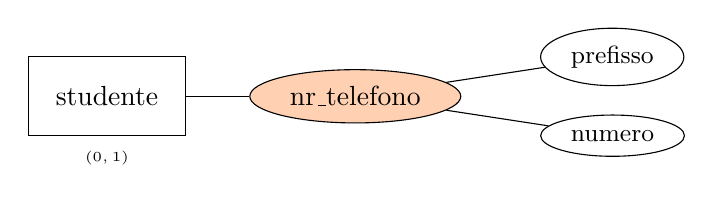
\begin{tikzpicture}[node distance=0.8cm]
				\node[rectangle, draw, minimum width=2cm, minimum height=1cm] (studente) {studente};
				\node[ellipse, draw, fill=orange!30, right=of studente] (tel) {nr\_telefono};
				\node[ellipse, draw, right=1cm of tel, yshift=0.5cm] (pref) {\small prefisso};
				\node[ellipse, draw, right=1cm of tel, yshift=-0.5cm] (num) {\small numero};
				
				\draw (studente) -- (tel);
				\draw (tel) -- (pref);
				\draw (tel) -- (num);
				
				\node[below=2pt of studente, font=\tiny] {$(0,1)$};
			\end{tikzpicture}
		\end{center}
		
		Si scompone in: \texttt{tel\_prefisso} e \texttt{tel\_numero}
	\end{frame}
	
	% Slide 18
	\begin{frame}{Attributi Composti: Soluzione B}
		\textbf{Soluzione B: non considerazione}
		
		\vspace{0.3cm}
		
		\begin{center}
			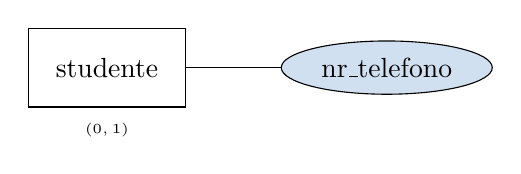
\begin{tikzpicture}
				\node[rectangle, draw, minimum width=2cm, minimum height=1cm] (studente) {studente};
				\node[ellipse, draw, fill=lightblue!30, right=1.2cm of studente] (tel) {nr\_telefono};
				
				\draw (studente) -- (tel);
				
				\node[below=2pt of studente, font=\tiny] {$(0,1)$};
			\end{tikzpicture}
		\end{center}
		
		Si mantiene come unico attributo: \texttt{nr\_telefono}
	\end{frame}
	
	% Slide 19
	\begin{frame}{Eliminazione Attributi Multivalore}
		Gli eventuali \textbf{attributi multivalore} presenti devono essere \textcolor{orange}{\textbf{"promossi" a entità}}.
		
		\vspace{0.5cm}
		
		Si crea una \textit{nuova entità} che contiene i valori dell'attributo e la si collega all'entità che possedeva l'attributo mediante una nuova relazione \textbf{uno-a-molti} o \textbf{molti-a-molti}, a seconda dei casi.
	\end{frame}
	
	% Slide 20
	\begin{frame}{Attributi Multivalore: Esempio 1}
		\textbf{Esempio:} Uno studente può parlare più di una lingua.
		
		\vspace{0.2cm}
		\begin{center}
			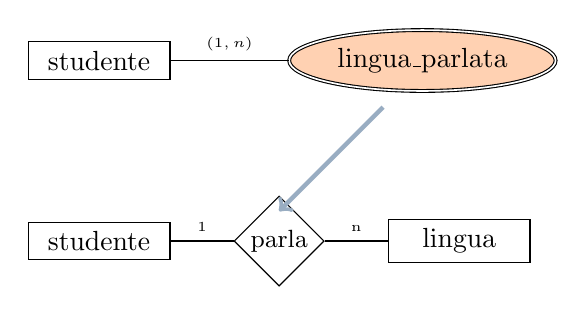
\begin{tikzpicture}[node distance=1.5cm]
				% Prima
				\node[rectangle, draw, minimum width=1.8cm] (stud1) {studente};
				\node[ellipse, draw, fill=orange!30, double, right=of stud1] (lingua1) {lingua\_parlata};
				\draw (stud1) -- node[above, font=\tiny] {$(1,n)$} (lingua1);
				
				% Dopo
				\node[rectangle, draw, minimum width=1.8cm, below=1.8cm of stud1] (stud2) {studente};
				\node[diamond, draw, right=0.8cm of stud2, inner sep=1pt, font=\small] (parla) {parla};
				\node[rectangle, draw, minimum width=1.8cm, right=0.8cm of parla] (lingua2) {lingua};
				
				\draw (stud2) -- node[above, font=\tiny] {1} (parla);
				\draw (parla) -- node[above, font=\tiny] {n} (lingua2);
				
				\draw[->, ultra thick, darkblue!40] ($(lingua1.south)-(0.5,0.2)$) -- ($(parla.north)-(0,0.2)$);
			\end{tikzpicture}
		\end{center}
	\end{frame}
	
	% Slide 21
	\begin{frame}{Attributi Multivalore: Esempio 2}
		\textbf{Esempio:} Un'azienda può possedere più numeri di telefono.
		
		\vspace{0.2cm}
		\begin{center}
			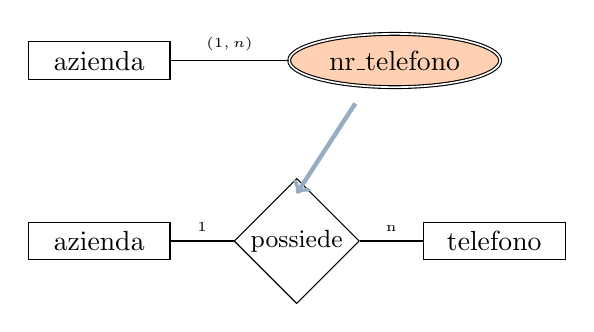
\begin{tikzpicture}[node distance=1.5cm]
				% Prima
				\node[rectangle, draw, minimum width=1.8cm] (az1) {azienda};
				\node[ellipse, draw, fill=orange!30, double, right=of az1] (tel1) {nr\_telefono};
				\draw (az1) -- node[above, font=\tiny] {$(1,n)$} (tel1);
				
				% Dopo
				\node[rectangle, draw, minimum width=1.8cm, below=1.8cm of az1] (az2) {azienda};
				\node[diamond, draw, right=0.8cm of az2, inner sep=1pt, font=\small] (poss) {possiede};
				\node[rectangle, draw, minimum width=1.8cm, right=0.8cm of poss] (tel2) {telefono};
				
				\draw (az2) -- node[above, font=\tiny] {1} (poss);
				\draw (poss) -- node[above, font=\tiny] {n} (tel2);
				
				\draw[->, ultra thick, darkblue!40] ($(tel1.south)-(0.5,0.2)$) -- ($(poss.north)-(0,0.2)$);
			\end{tikzpicture}
		\end{center}
	\end{frame}
	
	% Slide 22
	\begin{frame}{Attributi Multivalore: Esempio 3}
		\begin{center}
			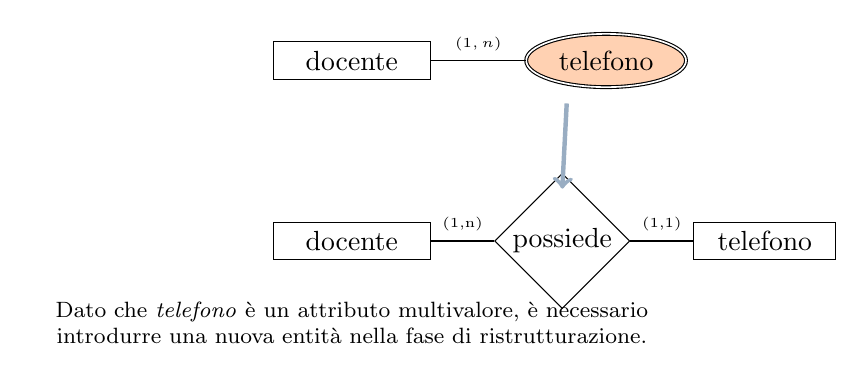
\begin{tikzpicture}[node distance=1.2cm]
				% Prima
				\node[rectangle, draw, minimum width=2cm] (doc1) {docente};
				\node[ellipse, draw, fill=orange!30, double, right=of doc1] (tel1) {telefono};
				\draw (doc1) -- node[above, font=\tiny] {$(1,n)$} (tel1);
				
				% Dopo
				\node[rectangle, draw, minimum width=2cm, below=1.8cm of doc1] (doc2) {docente};
				\node[diamond, draw, right=0.8cm of doc2, inner sep=1pt] (poss) {possiede};
				\node[rectangle, draw, minimum width=1.8cm, right=0.8cm of poss] (tel2) {telefono};
				
				\draw (doc2) -- node[above, font=\tiny] {(1,n)} (poss);
				\draw (poss) -- node[above, font=\tiny] {(1,1)} (tel2);
				
				\draw[->, ultra thick, darkblue!40] ($(tel1.south)-(0.5,0.2)$) -- ($(poss.north)-(0,0.2)$);
				
				\node[below=0.4cm of doc2, text width=8cm, align=center, font=\footnotesize] {Dato che \textit{telefono} è un attributo multivalore, è necessario introdurre una nuova entità nella fase di ristrutturazione.};
			\end{tikzpicture}
		\end{center}
	\end{frame}
	
	\section{Eliminazione Gerarchie}
	
	% Slide 23
	\begin{frame}{Eliminazione Gerarchie e Specializzazioni}
		La \textbf{gerarchia di generalizzazione} deve essere trasformata in una unica entità in quanto non è supportata dal modello relazionale.
		
		\vspace{0.5cm}
		
		È possibile ristrutturare il diagramma in due modi differenti:
		\begin{enumerate}
			\item \textcolor{darkblue}{\textbf{Eliminazione dei figli}} (collasso dei figli), aggiungendo uno o più attributi nell'entità padre
			\item \textcolor{orange}{\textbf{Eliminazione del padre}} (esplosione dei figli): completando ciascun figlio con gli attributi del padre
		\end{enumerate}
	\end{frame}
	
	% Slide 24
	\begin{frame}{Gerarchia: Esempio}
		\begin{center}
			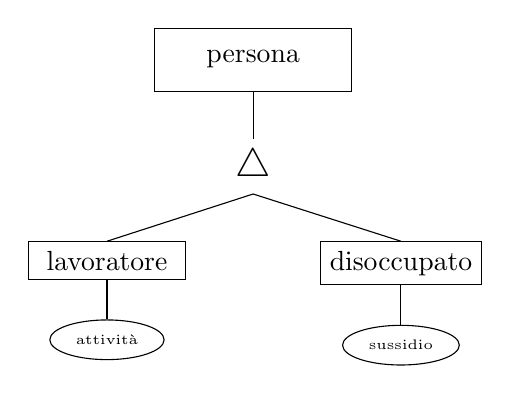
\begin{tikzpicture}[node distance=1cm]
				\node[rectangle, draw, minimum width=2.5cm, minimum height=0.8cm] (persona) {persona};
				\node[below=0.6cm of persona, font=\Large] (tri) {$\triangle$};
				
				\node[rectangle, draw, below left=0.6cm and 0.5cm of tri, minimum width=2cm] (lav) {lavoratore};
				\node[rectangle, draw, below right=0.6cm and 0.5cm of tri, minimum width=2cm] (dis) {disoccupato};
				
				\node[ellipse, draw, below=0.5cm of lav, font=\tiny] (att) {attività};
				\node[ellipse, draw, below=0.5cm of dis, font=\tiny] (sus) {sussidio};
				
				\draw (persona) -- (tri);
				\draw (tri.south) -- (lav.north);
				\draw (tri.south) -- (dis.north);
				\draw (lav) -- (att);
				\draw (dis) -- (sus);
			\end{tikzpicture}
		\end{center}
	\end{frame}
	
	% Slide 25
	\begin{frame}{Soluzione A: Collasso dei Figli}
		\textbf{Caso A:} Una sola entità con attributi opzionali.
		
		\begin{center}
			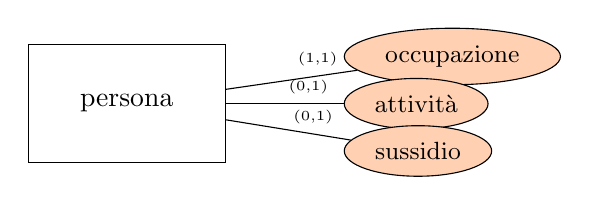
\begin{tikzpicture}[node distance=0.7cm]
				\node[rectangle, draw, minimum width=2.5cm, minimum height=1.5cm] (persona) {persona};
				\node[ellipse, draw, fill=orange!30, right=1.5cm of persona, yshift=0.6cm, font=\small] (occ) {occupazione};
				\node[ellipse, draw, fill=orange!30, right=1.5cm of persona, font=\small] (att) {attività};
				\node[ellipse, draw, fill=orange!30, right=1.5cm of persona, yshift=-0.6cm, font=\small] (sus) {sussidio};
				
				\draw (persona) -- node[above, pos=0.7, font=\tiny] {(1,1)} (occ);
				\draw (persona) -- node[above, pos=0.7, font=\tiny] {(0,1)} (att);
				\draw (persona) -- node[above, pos=0.7, font=\tiny] {(0,1)} (sus);
			\end{tikzpicture}
		\end{center}
	\end{frame}
	
	% Slide 26
	\begin{frame}{Soluzione B: Esplosione dei Figli}
		\textbf{Caso B:} Due entità distinte.
		
		\begin{center}
			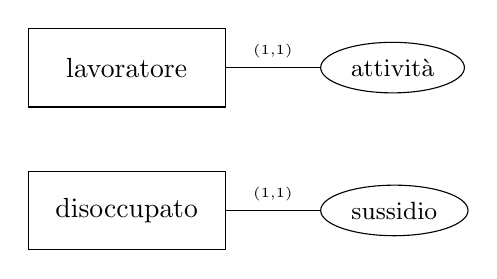
\begin{tikzpicture}[node distance=1.2cm]
				\node[rectangle, draw, minimum width=2.5cm, minimum height=1cm] (lav) {lavoratore};
				\node[ellipse, draw, right=of lav, font=\small] (att) {attività};
				\draw (lav) -- node[above, font=\tiny] {(1,1)} (att);
				
				\node[rectangle, draw, minimum width=2.5cm, minimum height=1cm, below=0.8cm of lav] (dis) {disoccupato};
				\node[ellipse, draw, right=of dis, font=\small] (sus) {sussidio};
				\draw (dis) -- node[above, font=\tiny] {(1,1)} (sus);
			\end{tikzpicture}
		\end{center}
	\end{frame}
	
	\section{Traduzione al Modello Relazionale}
	
	% Slide 27
	\begin{frame}{Traduzione: Panoramica}
		Dopo aver applicato al modello E-R le regole di ristrutturazione si ottiene lo \textbf{schema E-R ristrutturato}, pronto per essere trasformato nello schema relazionale.
		
		\vspace{0.5cm}
		
		In questa fase, che prende il nome di \textcolor{orange}{\textbf{fase di traduzione}}, vengono applicate le regole di trasformazione di entità, attributi e associazioni dello schema E-R in relazioni del modello relazionale.
	\end{frame}
	
	% Slide 28
	\begin{frame}{Traduzione delle Entità}
		Per ogni \textbf{entità} viene generata una \textcolor{darkblue}{\textbf{tabella}} indicando il suo \textit{schema relazionale}, dove viene riportato un \textbf{campo} per ogni \textbf{attributo} dell'entità.
		
		\begin{center}
			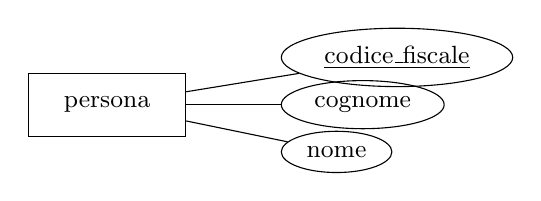
\begin{tikzpicture}[node distance=0.8cm, every node/.style={font=\small}]
				\node[rectangle, draw, minimum width=2cm, minimum height=0.8cm] (persona) {persona};
				\node[ellipse, draw, right=1.2cm of persona, yshift=0.6cm] (cf) {\underline{codice\_fiscale}};
				\node[ellipse, draw, right=1.2cm of persona] (cog) {cognome};
				\node[ellipse, draw, right=1.2cm of persona, yshift=-0.6cm] (nom) {nome};
				
				\draw (persona) -- (cf);
				\draw (persona) -- (cog);
				\draw (persona) -- (nom);
			\end{tikzpicture}
		\end{center}
		
		\begin{block}{Schema Relazionale}
			\texttt{persona (\underline{codice\_fiscale}, cognome, nome)}
		\end{block}
	\end{frame}
	
	% Slide 29
	\begin{frame}{Attributi Calcolati}
		In caso di presenza di \textbf{attributi calcolati} va aggiunto un vincolo di integrità che specifica il metodo di calcolo.
		
		\vspace{0.5cm}
		
		\begin{example}
			Un caso frequente è l'attributo \texttt{età}: questo viene calcolato come differenza di due date (data odierna e data di nascita), e se manca il valore di una di esse il suo valore deve essere \texttt{NULL}.
		\end{example}
	\end{frame}
	
	\section{Traduzione delle Relazioni}
	
	% Slide 30
	\begin{frame}{Trasformazione delle Relazioni}
		Si effettua la traduzione delle relazioni, in base a:
		\begin{itemize}
			\item Numero di entità partecipanti
			\item Loro cardinalità
		\end{itemize}
		
		\vspace{0.5cm}
		
		Tipologie:
		\begin{enumerate}
			\item Relazioni uno-a-uno (1,1)
			\item Relazioni uno-a-molti (1,N)
			\item Relazioni molti-a-molti (N,N)
			\item Relazioni ternarie
		\end{enumerate}
	\end{frame}
	
	% Slide 31
	\begin{frame}{Relazioni Uno-a-Uno (1,1)}
		Due entità legate da una relazione (1,1) possono essere \textcolor{orange}{\textbf{ridotte a un'unica entità}} che contiene gli attributi sia della prima sia della seconda entità.
		
		\begin{center}
			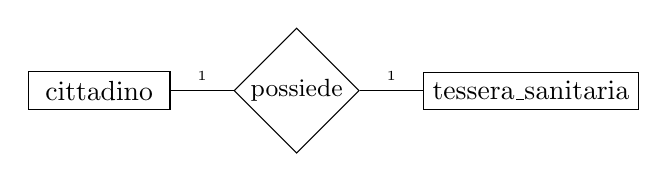
\begin{tikzpicture}
				\node[rectangle, draw, minimum width=1.8cm] (citt) {cittadino};
				\node[diamond, draw, right=0.8cm of citt, inner sep=1pt, font=\small] (poss) {possiede};
				\node[rectangle, draw, right=0.8cm of poss] (tess) {tessera\_sanitaria};
				
				\draw (citt) -- node[above, font=\tiny] {1} (poss);
				\draw (poss) -- node[above, font=\tiny] {1} (tess);
			\end{tikzpicture}
		\end{center}
		
		\vspace{0.2cm}
		\footnotesize
		La relazione è del tipo 1,1: un cittadino possiede una sola tessera e viceversa. La relazione è eliminabile e otteniamo un'unica entità con tutti gli attributi.
	\end{frame}
	
	% Slide 32
	\begin{frame}{Relazioni Uno-a-Uno: Risultato}
		\begin{center}
			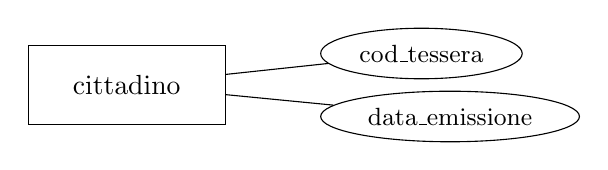
\begin{tikzpicture}
				\node[rectangle, draw, minimum width=2.5cm, minimum height=1cm] (citt) {cittadino};
				\node[ellipse, draw, right=1.2cm of citt, yshift=0.4cm, font=\small] (cod) {cod\_tessera};
				\node[ellipse, draw, right=1.2cm of citt, yshift=-0.4cm, font=\small] (dat) {data\_emissione};
				
				\draw (citt) -- (cod);
				\draw (citt) -- (dat);
			\end{tikzpicture}
		\end{center}
		
		Gli attributi della tessera sanitaria vengono incorporati nell'entità cittadino.
	\end{frame}
	
	% Slide 33
	\begin{frame}{Relazioni Uno-a-Molti (1,N)}
		Ogni associazione \textbf{uno a molti} può essere tradotta inserendo un \textcolor{orange}{\textbf{attributo aggiuntivo}} sulla entità da cui la cardinalità massima è 1.
		
		\vspace{0.5cm}
		
		Tale attributo conterrà la \textit{chiave dell'oggetto associato} all'oggetto corrente. Si introduce così una \textcolor{darkblue}{\textbf{chiave esterna (foreign key)}} e, con essa, un vincolo di integrità referenziale.
	\end{frame}
	
	% Slide 34
	\begin{frame}{Relazioni 1-N: Esempio}
		\begin{center}
			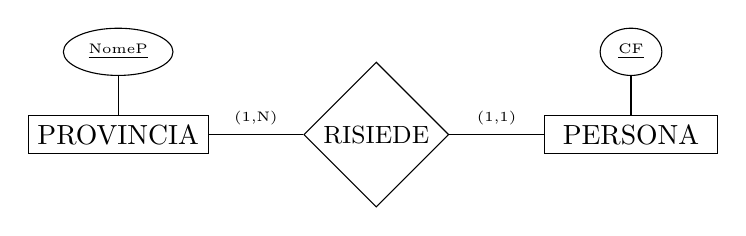
\begin{tikzpicture}[node distance=1.2cm]
				\node[rectangle, draw, minimum width=2.2cm] (prov) {PROVINCIA};
				\node[diamond, draw, right=of prov, inner sep=2pt, font=\small] (ris) {RISIEDE};
				\node[rectangle, draw, right=of ris, minimum width=2.2cm] (pers) {PERSONA};
				
				\draw (prov) -- node[above, font=\tiny] {(1,N)} (ris);
				\draw (ris) -- node[above, font=\tiny] {(1,1)} (pers);
				
				\node[ellipse, draw, above=0.5cm of prov, font=\tiny] (p1) {\underline{NomeP}};
				\node[ellipse, draw, above=0.5cm of pers, font=\tiny] (p2) {\underline{CF}};
				\draw (prov) -- (p1);
				\draw (pers) -- (p2);
			\end{tikzpicture}
		\end{center}
		
		\begin{block}{Schema Relazionale}
			\small
			\texttt{PROVINCIA(\underline{NomeP}, ...)} \\
			\texttt{PERSONA(\underline{CF}, Nome, \textit{NomeP}, Dal)} \\
			\texttt{FK: NomeP REFERENZIA PROVINCIA}
		\end{block}
	\end{frame}
	
	% Slide 35
	\begin{frame}{Relazioni Molti-a-Molti (N,N)}
		Le relazioni \textbf{N,N} non possono essere rappresentate nel modello logico relazionale.
		
		\vspace{0.5cm}
		
		Devono essere tradotte aggiungendo un'\textcolor{orange}{\textbf{entità associativa}} (anche detta entità "ponte") che va messa in relazione con le due entità originali.
	\end{frame}
	
	% Slide 36
	\begin{frame}{Relazioni N-N: Traduzione}
		Una relazione molti a molti che lega due entità si traduce in:
		\begin{itemize}
			\item Una \textbf{tabella per ogni entità} contenente gli attributi dell'entità
			\item Una \textbf{tabella per la relazione} contenente:
			\begin{itemize}
				\item Gli attributi identificatori delle entità che collega
				\item Gli attributi propri
			\end{itemize}
			\item Gli attributi identificatori della tabella collegata alla relazione compongono la \textcolor{darkblue}{\textbf{chiave esterna}}
		\end{itemize}
	\end{frame}
	
	% Slide 37
	\begin{frame}{Relazioni N-N: Esempio Studente-Corso}
		\begin{center}
			\begin{tikzpicture}[node distance=1.2cm]
				\node[rectangle, draw, min width=1.8cm] (stud) {STUDENTE};
				\node[diamond, draw, right=of stud, inner sep=2pt, font=\small] (esame) {ESAME};
				\node[rectangle, draw, right=of esame, min width=1.8cm] (corso) {CORSO};
				
				\draw (stud) -- node[above, font=\tiny] {N} (esame);
				\draw (esame) -- node[above, font=\tiny] {N} (corso);
				
				\node[ellipse, draw, above=0.5cm of esame, font=\tiny] (a) {ANNO};
				\node[ellipse, draw, below=0.5cm of esame, font=\tiny] (v) {VOTO};
				\draw (esame) -- (a);
				\draw (esame) -- (v);
			\end{tikzpicture}
		\end{center}
		
		\begin{block}{Schema Relazionale}
			\footnotesize
			\texttt{Studente(\underline{Matricola}, Nome)} \quad \texttt{Corso(\underline{Codice}, Denominazione)} \\
			\texttt{Esame(\underline{\textit{Matricola}, \textit{Codice}}, Anno, Voto)}
		\end{block}
	\end{frame}
	
	% Slide 38
	\begin{frame}{Relazioni N-N: Esempio Impiegato-Progetto}
		\begin{center}
			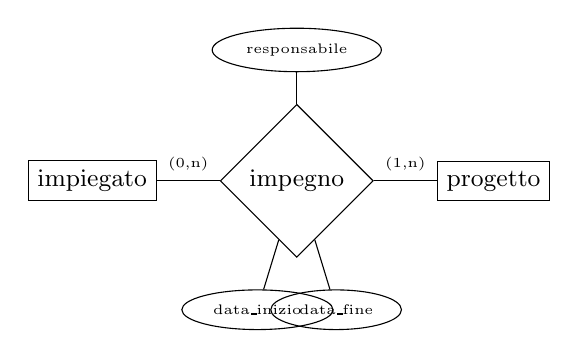
\begin{tikzpicture}[node distance=1cm, every node/.style={font=\tiny}]
				\node[rectangle, draw, minimum width=1.5cm, font=\small] (imp) {impiegato};
				\node[diamond, draw, right=0.8cm of imp, font=\small] (impegno) {impegno};
				\node[rectangle, draw, right=0.8cm of impegno, font=\small] (prog) {progetto};
				
				\draw (imp) -- node[above] {(0,n)} (impegno);
				\draw (impegno) -- node[above] {(1,n)} (prog);
				
				\node[ellipse, draw, above=0.4cm of impegno] (res) {responsabile};
				\node[ellipse, draw, below=0.4cm of impegno, xshift=0.5cm] (df) {data\_fine};
				\node[ellipse, draw, below=0.4cm of impegno, xshift=-0.5cm] (di) {data\_inizio};
				\draw (impegno) -- (res);
				\draw (impegno) -- (df);
				\draw (impegno) -- (di);
			\end{tikzpicture}
		\end{center}
		
		\begin{block}{Schema Relazionale}
			\footnotesize
			\texttt{impiegato (\underline{ID\_impiegato}, cognome, nome)} \\
			\texttt{progetto (\underline{ID\_progetto}, descrizione)} \\
			\texttt{impegno (\underline{\textit{ID\_impiegato}, \textit{ID\_progetto}}, data\_inizio, responsabile)}
		\end{block}
	\end{frame}
	
	\section{Relazioni Ternarie}
	
	% Slide 39
	\begin{frame}{Relazioni Ternarie}
		Una \textbf{relazione ternaria} collega logicamente tre entità.
		
		\begin{center}
			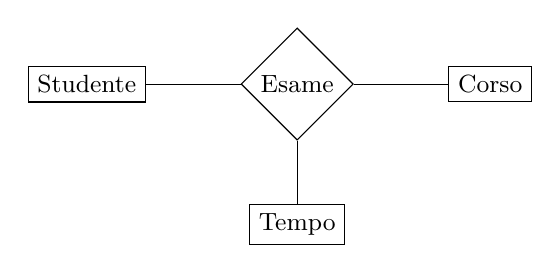
\begin{tikzpicture}[scale=0.8, every node/.style={font=\small}]
				\node[diamond, draw, inner sep=2pt] (esame) {Esame};
				\node[rectangle, draw, left=1.2cm of esame] (stud) {Studente};
				\node[rectangle, draw, right=1.2cm of esame] (corso) {Corso};
				\node[rectangle, draw, below=0.8cm of esame] (tempo) {Tempo};
				
				\draw (stud) -- (esame);
				\draw (corso) -- (esame);
				\draw (tempo) -- (esame);
			\end{tikzpicture}
		\end{center}
		
		\begin{example}
			Uno studente può ripetere lo stesso esame in tempi diversi.
		\end{example}
	\end{frame}
	
	% Slide 40
	\begin{frame}{Relazioni Ternarie: Caratteristiche}
		Le cardinalità minime raramente sono 1 per tutte le entità coinvolte in una relazione ternaria.
		
		\vspace{0.5cm}
		
		Le cardinalità massime di una relazione n-aria sono (praticamente) sempre \textbf{N}.
		
		\vspace{0.5cm}
		
		\begin{alertblock}{Nota importante}
			Se la partecipazione di un'entità E ha cardinalità massima 1, è possibile eliminare la relazione n-aria e legare l'entità E con le altre mediante relazioni binarie.
		\end{alertblock}
	\end{frame}
	
	% Slide 41
	\begin{frame}{Relazioni Ternarie: Esempio Fornitura}
		\begin{center}
			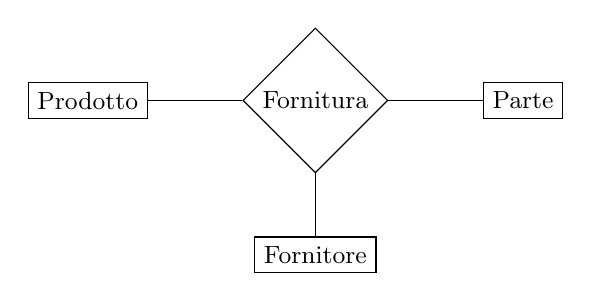
\begin{tikzpicture}[scale=0.8, every node/.style={font=\small}]
				\node[diamond, draw, inner sep=2pt] (forn) {Fornitura};
				\node[rectangle, draw, left=1.2cm of forn] (dip) {Prodotto};
				\node[rectangle, draw, right=1.2cm of forn] (prod) {Parte};
				\node[rectangle, draw, below=0.8cm of forn] (vend) {Fornitore};
				
				\draw (dip) -- (forn);
				\draw (prod) -- (forn);
				\draw (vend) -- (forn);
			\end{tikzpicture}
		\end{center}
		\footnotesize
		\begin{itemize}
			\item Il venditore A fornisce stampanti al Dipartimento Personale
			\item Il venditore B fornisce fotocopiatrici al Dipartimento Ricerca
		\end{itemize}
	\end{frame}
	
	% Slide 42
	\begin{frame}{Relazioni Ternarie: Traduzione}
		La relazione ternaria con cardinalità molti a molti viene trasformata nel seguente modo:
		\begin{itemize}
			\item Ogni \textbf{entità} in una tabella
			\item La \textbf{relazione} in una tabella contenente:
			\begin{itemize}
				\item Tutti gli attributi chiave delle entità collegate
				\item L'attributo proprio (se presente)
			\end{itemize}
		\end{itemize}
	\end{frame}
	
	% Slide 43
	\begin{frame}{Relazioni Ternarie: Schema Finale}
		\begin{block}{Schema Relazionale}
			\small
			\texttt{Prodotto(\underline{CodProd}, Nome)} \\
			\texttt{Fornitore(\underline{CodForn}, Telefono)} \\
			\texttt{Parte(\underline{CodPart}, Descrizione)} \\
			\texttt{Fornitura(\underline{\textit{CodPart}, \textit{CodProd}, \textit{CodForn}}, Quantità)}
		\end{block}
	\end{frame}
	
	% Slide 44
	\begin{frame}{Esempio Complesso: Fattura-Cliente-Prodotto}
		\begin{center}
			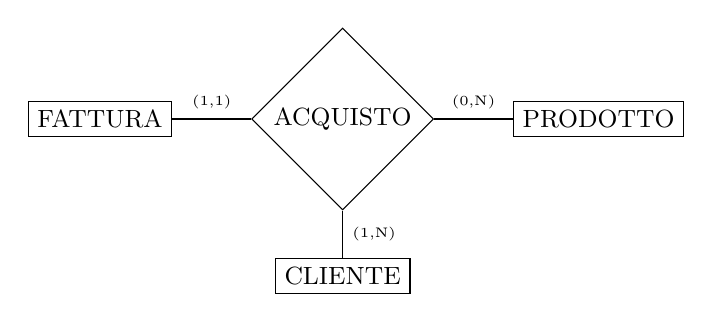
\begin{tikzpicture}[scale=0.8, every node/.style={font=\small}]
				\node[diamond, draw, inner sep=2pt] (acq) {ACQUISTO};
				\node[rectangle, draw, left=1cm of acq] (fatt) {FATTURA};
				\node[rectangle, draw, right=1cm of acq] (prod) {PRODOTTO};
				\node[rectangle, draw, below=0.6cm of acq] (cli) {CLIENTE};
				
				\draw (fatt) -- node[above, font=\tiny] {(1,1)} (acq);
				\draw (prod) -- node[above, font=\tiny] {(0,N)} (acq);
				\draw (cli) -- node[right, font=\tiny] {(1,N)} (acq);
			\end{tikzpicture}
		\end{center}
		\footnotesize
		La relazione ternaria con una cardinalità (1,1) può essere scomposta in relazioni binarie.
	\end{frame}
	
	% Slide 45
	\begin{frame}{Scomposizione Relazione Ternaria}
		\begin{center}
			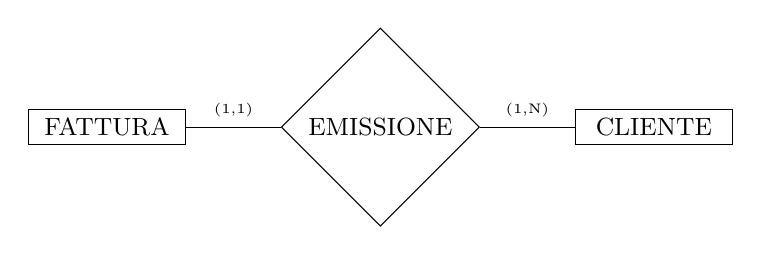
\begin{tikzpicture}[node distance=1.2cm, every node/.style={font=\small}]
				\node[rectangle, draw, minimum width=2cm] (fatt) {FATTURA};
				\node[diamond, draw, right=of fatt] (emis) {EMISSIONE};
				\node[rectangle, draw, right=of emis, minimum width=2cm] (cli) {CLIENTE};
				
				\draw (fatt) -- node[above, font=\tiny] {(1,1)} (emis);
				\draw (emis) -- node[above, font=\tiny] {(1,N)} (cli);
			\end{tikzpicture}
		\end{center}
	\end{frame}
	
	\section{Relazioni Ridondanti}
	
	% Slide 46
	\begin{frame}{Eliminare le Relazioni Ridondanti}
		Una \textbf{relazione ridondante} è una relazione definita tra due entità e che è equivalente nel significato a un'altra relazione tra le stesse due entità che passa attraverso un'entità intermedia.
		
		\vspace{0.4cm}
		\begin{example}
			\begin{itemize}
				\item Una persona abita in una provincia
				\item Una persona risiede in un paese
				\item Il paese si trova in una provincia
			\end{itemize}
		\end{example}
		La prima relazione è \textcolor{red}{ridondante} rispetto alle altre due.
	\end{frame}
	
	% Slide 47
	\begin{frame}{Ridondanza: Esempio Visivo}
		\begin{center}
			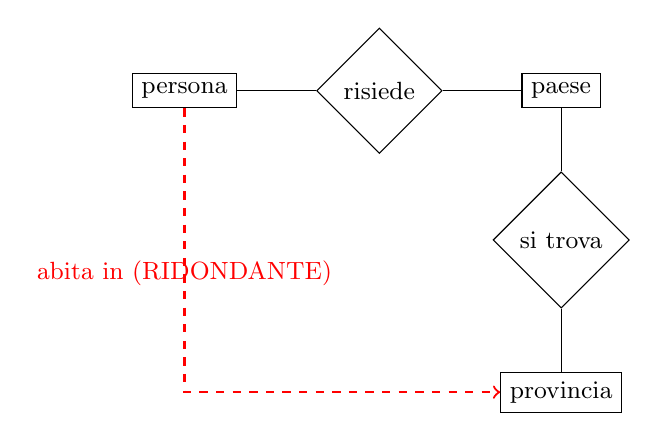
\begin{tikzpicture}[node distance=1cm, every node/.style={font=\small}]
				\node[rectangle, draw] (pers) {persona};
				\node[diamond, draw, right=of pers] (ris) {risiede};
				\node[rectangle, draw, right=of ris] (paese) {paese};
				\node[diamond, draw, below=0.8cm of paese] (trova) {si trova};
				\node[rectangle, draw, below=0.8cm of trova] (prov) {provincia};
				
				\draw (pers) -- (ris);
				\draw (ris) -- (paese);
				\draw (paese) -- (trova);
				\draw (trova) -- (prov);
				
				% Relazione ridondante
				\draw[red, dashed, thick, ->] (pers.south) |- node[below, pos=0.25] {abita in (RIDONDANTE)} (prov.west);
			\end{tikzpicture}
		\end{center}
	\end{frame}
	
	% Slide 48
	\begin{frame}{Definizione delle Chiavi}
		Aggiungere anche la definizione delle chiavi:
		\begin{itemize}
			\item Le \textbf{chiavi artificiali} iniziano con \texttt{ID}
			\item Per convenzione usiamo \texttt{ID} \textit{maiuscolo} per la chiave primaria
			\item Indichiamo con \texttt{id} \textit{minuscolo} le chiavi esterne
		\end{itemize}
		
		\vspace{0.5cm}
		
		\begin{example}
			\texttt{STUDENTE(\underline{ID\_studente}, nome, cognome, \textit{id\_classe})} \\
			\texttt{CLASSE(\underline{ID\_classe}, sezione, anno)}
		\end{example}
	\end{frame}
	
	% Slide 49
	\begin{frame}{Vincoli da Considerare}
		\begin{enumerate}
			\item Vincoli \textbf{NOT NULL} per gli attributi obbligatori
			\item Vincoli di \textbf{interdipendenza} di valori nulli
			\item Vincoli di \textbf{chiave} (primarie e non)
			\item Vincoli di \textbf{foreign key} che provengono dalla traduzione di relazioni
			\item Vincoli di \textbf{generalizzazione}, formulati come vincoli insiemistici
		\end{enumerate}
	\end{frame}
	
	% Slide 50
	\begin{frame}{Vincoli di Cardinalità}
		\begin{block}{Partecipazione obbligatoria (cardinalità minima 1)}
			Diventa vincolo di inclusione o foreign key dalla relazione che corrisponde all'entità verso quella che corrisponde alla ER-relazione
		\end{block}
		
		\vspace{0.3cm}
		
		\begin{block}{Funzionalità (cardinalità massima 1)}
			Diventa vincolo di chiave sulla relazione che corrisponde alla ER-relazione
		\end{block}
	\end{frame}
	
	% Final slide
	\begin{frame}[plain]
		\begin{center}
			\Huge \textcolor{darkblue}{Grazie per l'attenzione!}
			\vspace{2cm}
			
			\Large Domande?
		\end{center}
	\end{frame}
	
\end{document}